\section{Related Work}
\label{sec:relat}

\subsection{Vision Foundation Model}
% \noindent Vision foundation models aim to unify diverse visual tasks within a single framework. Early sequence-to-sequence approaches, such as Pix2Seq~\cite{chen2022unified}, Unified-IO~\cite{lu2022unifiedio}, and OFA~\cite{wang2022ofa}, reformulated vision problems as sequence prediction and instruction-based learning. Later methods, including UViM~\cite{zhang2022uvim} and Uni-Perceiver~\cite{zhu2022uniperceiver}, introduced task-agnostic interfaces for multimodal understanding. Recent advances leverage stronger backbones and generative paradigms, e.g. Florence-2~\cite{xiao2023florence2}, InstructCV~\cite{gan2023instructcv}, and InstructDiffusion~\cite{geng2023instructdiffusion}, enabling prompt-driven recognition and conditional generation under a unified architecture.

% Most notably, VLMs have emerged as unified frameworks that couple visual encoders with large language models under instruction-driven settings. Emu ~\cite{sun2023emu, wang2024emu3} series integrate diffusion models with LLM-predicted embeddings, functioning as a generalist model capable of handling diverse vision tasks. Chameleon~\cite{chameleon2024} team follows an early-fusion strategy, integrating text and image tokens from the outset to support interleaved understanding and generation. In contrast, Transfusion~\cite{transfusion2024} combines next-token prediction for language with diffusion for images, and Show-o~\cite{showo2024} extends this hybrid approach with a one-transformer design that merges auto-regression and discrete diffusion. Collectively, these efforts highlight the trend of VLMs shaping the evolution of vision generalist models.

\noindent Vision foundation models aim to unify diverse visual tasks within a single framework. Early approaches reformulated vision problems as sequence prediction or instruction-based learning (Pix2Seq~\cite{chen2022unified}, Unified-IO~\cite{lu2022unifiedio}, OFA~\cite{wang2022ofa}), while later works introduced task-agnostic multimodal interfaces (UViM~\cite{zhang2022uvim}, Uni-Perceiver~\cite{zhu2022uniperceiver}). Recent advances further leverage stronger multimodal backbones and instruction-driven paradigms for prompt-based recognition and conditional generation (Florence-2~\cite{xiao2023florence2}, InstructCV~\cite{gan2023instructcv}, InstructDiffusion~\cite{geng2023instructdiffusion}). Meanwhile, VLMs have emerged as powerful vision generalists through unified multimodal architectures, including Emu~\cite{sun2023emu,wang2024emu3}, Chameleon~\cite{chameleon2024}, Transfusion~\cite{transfusion2024}, and Show-o~\cite{showo2024}. Collectively, these efforts highlight the trend of VLMs shaping the evolution of vision generalist models.

\subsection{Visual In-Context Learning}
Visual in-context learning (VICL) refers to adapting vision models to downstream tasks through contextual examples rather than explicit fine-tuning, and it can be broadly divided into visual prompting and prompt-driven conditioning. Implicit prompting methods, represented by MAE-VQGAN~\cite{bar2022visual} and Painter~\cite{wang2023painter}, rely on masked prediction or image completion as objectives, enabling models to generalize under diverse vision tasks. In contrast, explicit prompt-driven approaches leverage explicit conditioning to adapt diverse vision problems. For instance, Prompt Diffusion~\cite{wang2023incontext} exploits diffusion-based generation under prompt guidance. While PromptGIP~\cite{liu2023promptgip} adopts QA-style prompt structures. Additional works such as CoOp~\cite{zhou2022coop} and VPT ~\cite{jia2022vpt} further extend VICL by introducing learnable prompts for vision transformers. More recently, X-Prompt~\cite{xprompt2024universal} targets general image generation, compressing contextual signals and unifying diverse vision tasks within an auto-regressive framework. Most existing VICL methods focus on performing the visual prompt and query image in the same tasks, our T2T-VICL extends this paradigm to difficult cross-task settings, where the visual prompt and query image are from different tasks, digging the potential knowledge adaptation across diverse vision tasks.

\begin{figure*}[ht]
    \centering
    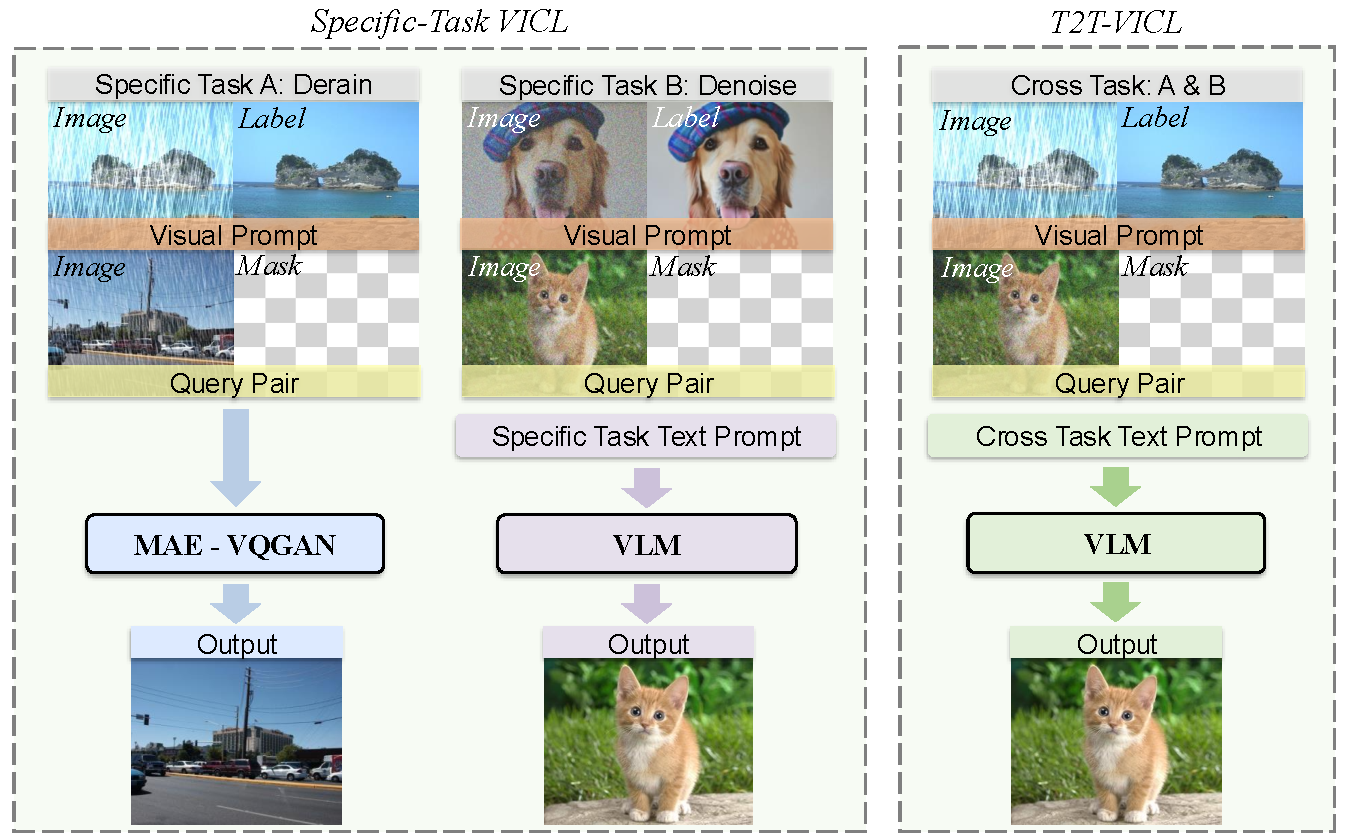
\includegraphics[width=0.9\textwidth]{fig/figure1vertical.pdf}
    \caption{Illustration of Cross-Task Visual In-Context Learning}
    \label{fig:fig1}
\vspace{-8pt}
\end{figure*}

\subsection{Task Transfer}
Task generalization refers to leveraging knowledge from previously solved tasks to facilitate learning on unseen ones. Early milestones such as Taskonomy ~\cite{zamir2018taskonomy} provided the first large-scale analysis of transferability across 26 vision tasks, introducing the task affinity matrix as a foundation for cross-task generalization. Following this line, TMT~\cite{pal2019tmt} extended Taskonomy by applying matrix factorization to refine the estimation of inter-task transferability. Similarly, Task2Vec~\cite{achille2019task2vec} proposed embedding tasks into a vector space using Fisher information, making task similarity measurable and interpretable. Beyond these foundations,~\cite{standley2020mtl} systematically investigated which tasks should be learned together in multitask settings, highlighting task affinity as a guiding principle. Paper~\cite {dwivedi2019crosstask} introduced cross-task consistency to enforce relational constraints. Given the growing visual generation ability of VLMs, the progress in this field motivates our exploration of cross-task generalization in VLMs and unlocks the boundaries.

\subsection{Language-Driven Image Editing}
\noindent Language-driven vision restoration has evolved from instruction-guided editing to adaptive prompt-based restoration. Early works such as InstructPix2Pix~\cite{brooks2023instructpix2pix}, InstructIR~\cite{conde2024instructir}, and PromptIR~\cite{potlapalli2023promptir} showed that natural language can guide fine-grained, degradation-aware manipulation of image features. Subsequent studies including SPIRE~\cite{qi2024spire}, PromptFix~\cite{yu2024promptfix}, Perceive-IR~\cite{zhang2025perceive}, and FPro~\cite{zhou2024fpro} further enriched semantic and perceptual prompting, enabling finer control over fidelity and restoration strength. These advances establish natural language as a direct and interpretable driver for low-level vision tasks.
